\documentclass[oneside, 11pt]{article}

\usepackage[T1]{fontenc}
\usepackage[utf8]{inputenc}
\usepackage[dutch]{babel}

\usepackage{fouriernc}
\usepackage[detect-all, load-configurations=binary,
            separate-uncertainty=true, per-mode=symbol,
            retain-explicit-plus, range-phrase={ tot }]{siunitx}

\usepackage{setspace}
\setstretch{1.2}

\setlength{\parskip}{\smallskipamount}
\setlength{\parindent}{0pt}

\usepackage{geometry}
\geometry{marginparwidth=0.5cm, verbose, a4paper, tmargin=3cm, bmargin=3cm, lmargin=2cm, rmargin=2cm}

\usepackage{float}

\usepackage[fleqn]{amsmath}
\numberwithin{equation}{section}
\numberwithin{figure}{section}

\usepackage{graphicx}
\graphicspath{{Figures/}}
\usepackage{subfig}

\usepackage{tikz}
\usetikzlibrary{plotmarks}

\usepackage{fancyhdr}
\pagestyle{fancy}
\fancyhf{}
\rhead{\thepage}
\renewcommand{\footrulewidth}{0pt}
\renewcommand{\headrulewidth}{0pt}

\usepackage{relsize}
\usepackage{xspace}
\usepackage{url}

\newcommand{\figref}[1]{Figuur~\ref{#1}}

\newcommand{\hisparc}{\textsmaller{HiSPARC}\xspace}
\newcommand{\kascade}{\textsmaller{KASCADE}\xspace}
\newcommand{\sapphire}{\textsmaller{SAPPHiRE}\xspace}
\newcommand{\jsparc}{\textsmaller{jSparc}\xspace}
\newcommand{\hdf}{\textsmaller{HDF5}\xspace}
\newcommand{\aires}{\textsmaller{AIRES}\xspace}
\newcommand{\csv}{\textsmaller{CSV}\xspace}
\newcommand{\python}{\textsmaller{PYTHON}\xspace}
\newcommand{\corsika}{\textsmaller{CORSIKA}\xspace}
\newcommand{\labview}{\textsmaller{LabVIEW}\xspace}
\newcommand{\daq}{\textsmaller{DAQ}\xspace}
\newcommand{\adc}{\textsmaller{ADC}\xspace}
\newcommand{\adcs}{\textsmaller{ADC}s\xspace}
\newcommand{\Adcs}{A\textsmaller{DC}s\xspace}
\newcommand{\hi}{\textsc{h i}\xspace}
\newcommand{\hii}{\textsc{h ii}\xspace}
\newcommand{\mip}{\textsmaller{MIP}\xspace}
\newcommand{\hisparcii}{\textsmaller{HiSPARC II}\xspace}
\newcommand{\hisparciii}{\textsmaller{HiSPARC III}\xspace}
\newcommand{\pmt}{\textsmaller{PMT}\xspace}
\newcommand{\pmts}{\textsmaller{PMT}s\xspace}

\DeclareSIUnit{\electronvolt}{\ensuremath{\mathrm{e\!\!\:V}}}

\DeclareSIUnit{\unitsigma}{\ensuremath{\sigma}}
\DeclareSIUnit{\mip}{\textsmaller{MIP}}
\DeclareSIUnit{\adc}{\textsmaller{ADC}}

\DeclareSIUnit{\gauss}{G}
\DeclareSIUnit{\parsec}{pc}
\DeclareSIUnit{\year}{yr}



\title{Checklist Installatie station}
\author{C.G.N. van Veen}
\docdetector{5}{CI}
\version{1.0}

\begin{document}

\maketitle

\section{Checklist}

De documenten `uitlijnen van de ADCs' , `inregelen van de PMTs' en 
`GPS calibratie' hebben U geholpen met de instellingen van de \hisparc
\daq. Dit document heeft tot doel om een laatste check te doen. Het
biedt een overzicht van de laatste belangrijke instellingen voordat U kunt gaan
meten/ data kan verzenden met het \hisparc station. 

\subsection{Data acquisitie modus}

\emph{U kunt de detector pas in gebruik nemen wanneer alle voorgaande procedures correct zijn uitgevoerd.}

De definitieve instellingen voor alle \hisparc detectorstations zijn als volgt.

\subsection{Time window instellingen}

In de \daq software klikt U op de \emph{Events / Settings} tab, klik op het 
tabje \emph{Time Window}. Als het goed is zijn de instellingen niet veranderd 
en staan ze nog als volgt. Zie \figref{fig:daq-time-window}:

\begin{itemize}
    \item Precoincidence time: 1 us
    \item Coincidence time: 1,5 us
    \item Post coincidence time: 3,5 us
\end{itemize}

\begin{figure}
    \centering
    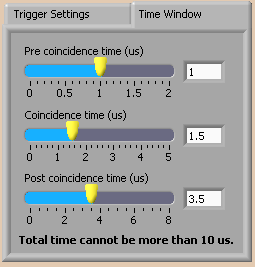
\includegraphics[scale=0.6]{daq-time-window}
    \caption{De instellingen voor het coïncidentie tijdvenster.}
    \label{fig:daq-time-window}
\end{figure}


\subsection{Opstelling met twee detectoren}

De instellingen voor stations met twee detectoren zijn als volgt. Zie
\figref{fig:daq-trigger-two-detectors}:


\begin{itemize}
    \item Threshold Low (alle kanalen): -30 mV
    \item Threshold High (alle kanalen): -70 mV
    \item Trigger: 2 low \textbf{AND} Don’t use high threshold \textbf{AND} Don’t use external trigger
\end{itemize}


\begin{figure}
    \centering
    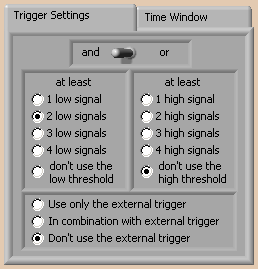
\includegraphics[scale=0.6]{daq-trigger-two-detectors}
    \caption{De triggerinstellingen voor een detectorstation met twee detectoren.}
    \label{fig:daq-trigger-two-detectors}
\end{figure}


\subsection{Opstelling met vier detectoren}

De instellingen voor stations met vier detectoren zijn als volgt. Zie
\figref{fig:daq-trigger-four-detectors}

\begin{itemize}
    \item Threshold Low (alle kanalen): -30 mV
    \item Threshold High (alle kanalen): -70 mV
    \item Trigger: 3 low \textbf{OR} 2 high \textbf{AND} Don’t use external trigger
\end{itemize}   

 
\begin{figure}
    \centering
    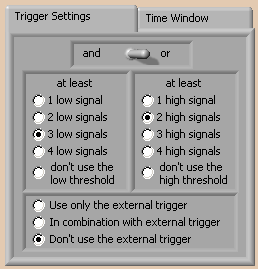
\includegraphics[scale=0.6]{daq-trigger-four-detectors}
    \caption{De triggerinstellingen voor een detectorstation met vier detectoren.}
    \label{fig:daq-trigger-four-detectors}
\end{figure}

\subsection{Automatisch opstarten in DAQ modus}

Iedere keer als het programma is opgestart kunt u op de knop \emph{Start DAQ}
mode klikken om over te gaan naar de data acquisitie modus. \emph{Alleen dan
wordt er daadwerkelijk data naar het Nikhef gestuurd!}

Om er voor te zorgen dat de detector na elke reboot automatisch opstart
in de data acquisitie modus gaat u naar de \emph{Expert Settings} tab en vinkt
u \emph{Start in DAQ} mode aan.

\begin{note}
Het is aan te bevelen de werking van de pc te testen door de pc nu
opnieuw op te starten. Als hij automatisch inlogt, het HiSPARC DAQ
programma start en automatisch overgaat naar de DAQ modus, is het meeste
werk gedaan. Controleert u alstublieft op \url{data.hisparc.nl}
of uw detectorstation volledig functioneert. Het kan ongeveer twintig
minuten duren voordat Nagios volledig geupdate is. Mocht er een foutmelding 
zijn. Dan kan het document `dagelijkse controle van een station' hulp bieden.
\end{note}


\subsection{HiSPARC Local Diagnostic Tool}

Om te controleren of de installatie succesvol is verlopen en alle
netwerkverbindingen zonder problemen werken is het van belang de \emph{Local
Diagnostic Tool} te draaien. Deze vindt u onder \emph{Start -> Alle
Programmma’s -> HiSPARC -> LocalDiagnosticTool of Start -> Programs ->
HiSPARC -> Status -> Diagnostics.}

\begin{figure}
    \centering
    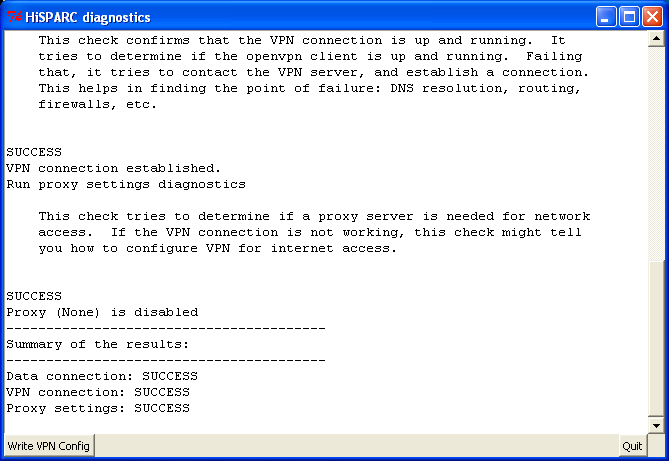
\includegraphics[scale=0.6]{localdiagnostictool}
    \caption{Screenshot van de Local Diagnostic Tool. Op deze PC is alles in orde, en er is geen proxy server vereist.}
    \label{fig:localdiagnostictool}
\end{figure}

Na opstarten van het programma verschijnt een wit tekstscherm waarin de
resultaten van een aantal controles worden weergegeven. De samenvatting
aan het eind moet overal \emph{SUCCESS} weergeven. Voor de beste instellingen,
klikt u op \emph{Write VPN config}, ook als alles in orde is. Is dit \emph{niet} het
geval, en staat er vlak boven de samenvatting iets als \emph{Proxy
(proxy01.server.example.com)} is enabled, klikt u dan op \emph{Write VPN
config}, herstart de pc en start u nogmaals de Local Diagnostic Tool. De
proxy instellingen zijn dan geschreven en er wordt van via die weg
geprobeerd verbinding te maken.

Bij aanhoudende problemen, kunt u in het witte venster klikken, en met
Ctrl-A alle tekst selecteren. Met Ctrl-C kopieert u het naar het
klembord. U kunt dan in een e-mail op Ctrl-V drukken en u heeft de
volledige uitvoer van de controles. U kunt uw mail sturen naar
\emph{beheer@hisparc.nl}. We zullen dan zo snel mogelijk contact met u opnemen.

\subsection{Monitor en controle}

De status van Uw station is te vinden op \url{data.hisparc.nl}, zoek Uw
station daar in de lijst. Het bolletje voor het station zou groen van
kleur moeten zijn. Is dat niet het geval dan kan het document
`dagelijkse controle van een station' wat ook in het infopakket van
\hisparc te vonden is, hulp bieden.


De clustercoördinatoren van \hisparc hebben bovendien de mogelijkheid om de
instellingen van de detector via een ‘virtual private network’ (VPN) op afstand 
te wijzigen. De toegang tot de pc’s biedt de mogelijkheid om snel en 
efficiënt kritische instellingen te veranderen en software updates door te voeren.

\begin{figure}
    \centering
    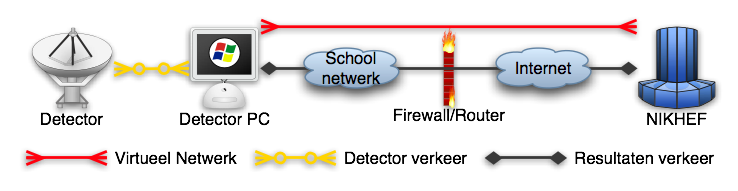
\includegraphics[scale=0.6]{network-diagram}
    \caption{De software biedt monitor en controle mogelijkheden via een VPN verbinding. Data van de detector wordt over een gescheiden verbinding verzonden.}
    \label{fig:network-diagram}
\end{figure}

\end{document}
